\documentclass[10pt, aspectratio=169, usepdftitle=false, draft]{beamer}

\usetheme[progressbar=frametitle]{metropolis}
\usepackage{appendixnumberbeamer} % Probably not needed

\usepackage[danish]{babel}

\usepackage{hyperref} %References

\hypersetup{
    pdftitle={SOP 2019 --- Præsentation},
    pdfauthor={Jens Tinggaard}
}

\usepackage{booktabs} % what is this?
\usepackage[scale=2]{ccicons} % and this?

\usepackage{pgfplots} % Do i need this?
\usepgfplotslibrary{dateplot}

\usepackage{xspace} % Or this?

\title{Studieområdeprojekt 2019}
\subtitle{Sikkerhed bag login-formular på en hjemmeside}
\date{27. januar 2020}
\author{Jens Tinggaard}
\institute{Odense Tekniske Gymnasium}
\titlegraphic{\hfill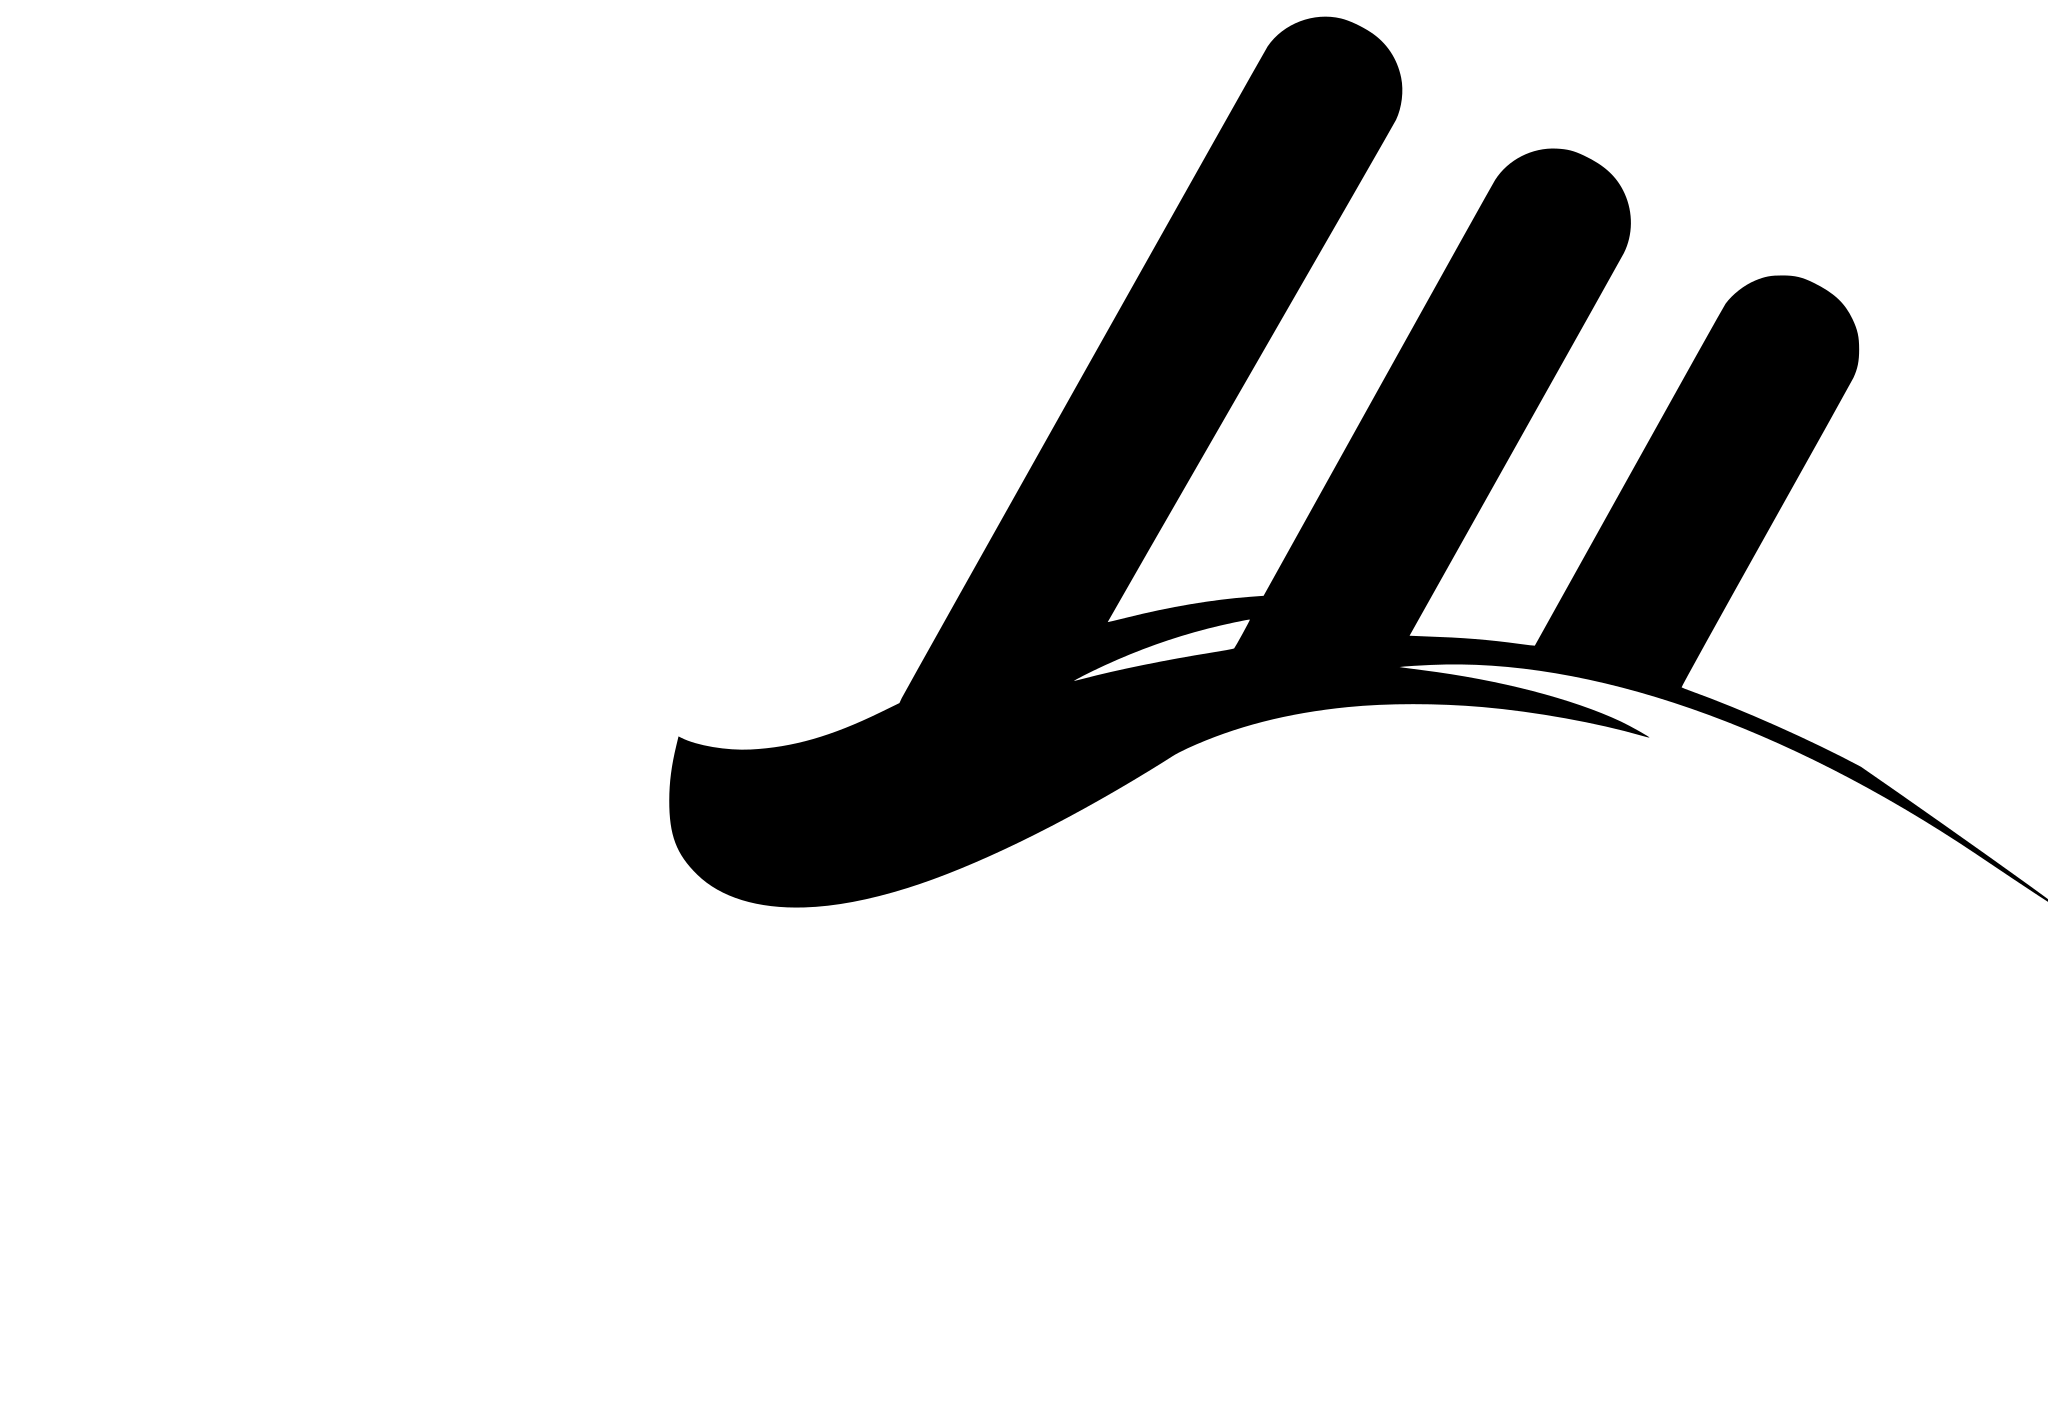
\includegraphics[height=1.5cm]{img/otg_logo.png}}



\begin{document}

\maketitle


\begin{frame}{Opgaveformulering}
\begin{itemize}
    \large
    \item Redegør for talteorien bag RSA kryptering. Forklar nødvendigheden af primtal og hvordan RSA metoden fungerer.
    \item Gør kort rede for hashing.
    \item Analyser forskellen på hashing og kryptografi og hvilken rolle de har i forhold til sikkerhed.
    \item Vurder hvorfor RSA er vigtigt i forbindelse med sikkerhed ved logins.
\end{itemize}
\end{frame}
%--- Next Frame ---%

\begin{frame}{Konklusion på projektet}
    \begin{itemize}
        \large
        \item Hvorfor RSA er så vigtig - hvor bruges det?
        \item Hvad RSA bygger på.
        \item Metoder som RSA og hashing bliver sjælendt brugt alene.
    \end{itemize}
\end{frame}
%--- Next Frame ---%

\begin{frame}{Relevante metoder i fagene}
    Matematik:
    \begin{enumerate}
        \item Talteori
        \item Beviser
        \item Vurdering \& Sammenligninger
    \end{enumerate}\pause
    Programmering:
    \begin{enumerate}
        \item Prototkoller
        \item Skitsering af id\'eer
        \item Dokumentationslæsning
    \end{enumerate}
\end{frame}
%--- Next Frame ---%

\begin{frame}{Empiri}
    Empiri
\end{frame}
%--- Next Frame ---%

\begin{frame}{Sammenspil mellem fagene}
    Sammenspil mellem fagene
\end{frame}
%--- Next Frame ---%

\begin{frame}{Kildekritik}
    Kildekritik
\end{frame}
%--- Next Frame ---%

\end{document}
